%\documentclass[12pt]{article}

\questionheader{ex:s3.1}

%%%%%%%%%%%%%%%%%%
\subsection*{\Conceptual}
%%%%%%%%%%%%%%%%%%
\begin{question}
Parametrize the surface given by $z=e^{x+1}+xy$ in terms of $x$ and $y$.
\end{question}
\begin{hint}
Your answer will have the form $\vr(x,y)= \psi_1(x,y)\hi+ \psi_2(x,y)\hj+ \psi_3(x,y)\hk$.
\end{hint}
\begin{answer}
 $\vr(x,y)= x\hi+ y\hj+ (e^{x+1}+xy)\hk$
\end{answer}
\begin{solution}
This parametrization is almost trivial. We know it will have the form $\vr(x,y)= \psi_1(x,y)\hi+ \psi_2(x,y)\hj+ \psi_3(x,y)\hk$ where $\psi_1$ gives the $x$-component (i.e. $x$), $\psi_2$ gives the $y$-component (i.e. $y$), and $\psi_3$ gives the $z$-component (i.e. $e^{x+1}+xy$). So,
 $\vr(x,y)= x\hi+ y\hj+ (e^{x+1}+xy)\hk$
\end{solution}
%%%%%%%%%%%%%%%%%%%
%\begin{question}
%Given a parametrization, describe the range
%\end{question}
%\begin{hint}
%\end{hint}
%\begin{answer}
%\end{answer}
%\begin{solution}
%\end{solution}
%%%%%%%%%%%%%%%%%%%
%\begin{question}
%Give a parametrization for a solid of rotation.
%\end{question}
%\begin{hint}
%\end{hint}
%\begin{answer}
%\end{answer}
%\begin{solution}
%\end{solution}
%%%%%%%%%%%%%%%%%%%
%\begin{question}
%Show two parametrizations give the same surface
%\end{question}
%\begin{hint}
%\end{hint}
%\begin{answer}
%\end{answer}
%\begin{solution}
%\end{solution}
%%%%%%%%%%%%%%%%%%%
%\begin{question}
%Fill-in-the-blank of a parametrization
%\end{question}
%\begin{hint}
%\end{hint}
%\begin{answer}
%\end{answer}
%\begin{solution}
%\end{solution}
%%%%%%%%%%%%%%%%%%


\begin{question}[M317 2010D]   %3b
Let $S$ be the surface given by
\begin{equation*}
\vr(u, v) = \big( u + v\,,\, u^2 + v^2 \,,\, u - v\big),\qquad
-2 \le u \le 2,\ -2 \le v \le 2
\end{equation*}
This is a surface you are familiar with. What surface is it (it may be 
just a portion of one of the following)? 
\begin{center}
sphere\quad\ 
helicoid\quad\ 
ellipsoid\quad\ 
saddle\quad\ 
parabolic bowl\quad\ 
cylinder\quad\ 
cone\quad\ 
plane
\end{center}
\end{question}

%\begin{hint} 
%
%\end{hint}

\begin{answer} 
      parabolic bowl
\end{answer}

\begin{solution} 
Our parametrization is
\begin{align*}
x(u,v) &= u+v \\
y(u,v) &= u^2+v^2 \\
z(u,v) &= u-v
\end{align*}
\begin{itemize}
\item
Adding $x(u,v)$ and $z(u,v)$ gives $x(u,v)+z(u,v) = 2u$. 
\item
Subtracting $z(u,v)$ from $x(u,v)$ gives $x(u,v)-z(u,v) = 2v$.
\end{itemize}
So $u=\frac{1}{2}\big(x(u,v)+z(u,v)\big)$ and
        $v=\frac{1}{2}\big(x(u,v)-z(u,v)\big)$. So on our surface
\begin{align*}
y(u,v) &= u^2+v^2 = \frac{1}{4}\big(x(u,v)+z(u,v)\big)^2
                  +\frac{1}{4}\big(x(u,v)-z(u,v)\big)^2 \\
 &= \frac{1}{2} x(u,v)^2 + \frac{1}{2} z(u,v)^2
\end{align*}
All points of our surface lie on $2y= x^2+z^2$. This is a parabolic bowl:
\begin{itemize}\itemsep1pt \parskip0pt \parsep0pt %\itemindent-15pt
\item[$\circ$]
no points have $y<0$ and
\item[$\circ$]
the $y=Y$ (with $Y> 0$) cross-section is the circle
$x^2+z^2=2Y$, $y=Y$
\item[$\circ$]
the $x=0$ cross-section is the parabola $2y=z^2$, $x=0$
\item[$\circ$]
the $z=0$ cross-section is the parabola $2y=x^2$, $z=0$
\end{itemize}

\begin{center}
       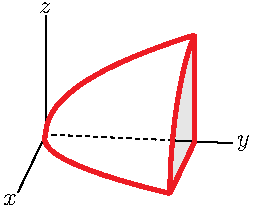
\includegraphics{parabolicBowl.pdf}
\end{center}

\end{solution}


%%%%%%%%%%%%%%%%%%
\subsection*{\Procedural}
%%%%%%%%%%%%%%%%%%

%\begin{question}
%Given a parametrization, describe the surface.
%\end{question}
%\begin{hint}
%\end{hint}
%\begin{answer}
%\end{answer}
%\begin{solution}
%\end{solution}
%%%%%%%%%%%%%%%%%%

%%%%%%%%%%%%%%%%%%%%%%%%%%%
\begin{question}[M317 2009A] %5
Suppose $S$ is the part of the hyperboloid $x^2 + y^2 - 2z^2 = 1$ 
that lies inside the cylinder $x^2 + y^2 = 9$ and above the plane $z = 1$ 
(i.e. for which $z \ge 1$).

Which of the following are parameterizations of $S$? 
%Write your answer 
%`yes' (Y) or `no' (N) in the following box.
%
%\begin{center}
%\begin{tabular}{ | c | c | c | c | c | c | }
%  \hline			
%      & 1 & 2 & 3 & 4 & 5 \\
%  \hline
%  Y/N & \phantom{N}  & \phantom{N} & \phantom{N} & \phantom{N} & \phantom{N} \\
%  \hline  
%\end{tabular}
%\end{center}

\begin{enumerate}[(a)]
\item  %1
The vector function 
\begin{equation*}
\vr(u,v) = u\,\hi  + v\,\hj +\frac{\sqrt{u^2+v^2-1}}{\sqrt{2}}\,\hk
\end{equation*}
with domain $D=\Set{(u,v)}{ 2 \le u^2+v^2 \le 9}$.


\item  %2
The vector function 
\begin{equation*}
\vr(u,v) = u\sin v\,\hi  - u\cos v\,\hj +\sqrt{\frac{u^2}{2}-\frac{1}{2}}\,\hk
\end{equation*}
with domain $D=\Set{(u,v)}{ \sqrt{3} \le u\le 3,\ 0\le v\le 2\pi}$.

\item  %3
The vector function 
\begin{equation*}
\vr(u,v) = \sqrt{1+2v^2}\cos u\,\hi  + \sqrt{1+2v^2} \sin u\,\hj +v\,\hk
\end{equation*}
with domain $D=\Set{(u,v)}{ 0\le u\le 2\pi,\ 1\le v\le 2}$.


\item  %4
The vector function 
\begin{equation*}
\vr(u,v) = \sqrt{1+u}\sin v\,\hi  + \sqrt{1+u} \cos v\,\hj 
                                  +\sqrt{\frac{u}{2}}\,\hk
\end{equation*}
with domain $D=\Set{(u,v)}{ 2\le u\le 8,\ 0\le v\le 2\pi}$.


\item  %5
The vector function 
\begin{equation*}
\vr(u,v) = \sqrt{u}\cos v\,\hi  - \sqrt{u} \sin v\,\hj 
                                  +\frac{\sqrt{u+1}}{\sqrt{2}}\,\hk
\end{equation*}
with domain $D=\Set{(u,v)}{ 3\le u\le 9,\ 0\le v\le 2\pi}$.

\end{enumerate}
\end{question}

\begin{hint} 
First think about what properties $\vr(u,v)$ has to have in order to be
a parametrization.
\end{hint}

\begin{answer} 
(a) No\qquad
(b) Yes\qquad
(c) Yes\qquad
(d) Yes\qquad
(e) No
\end{answer}

\begin{solution} 
Note that, since $x^2+y^2=1+2z^2$ on $S$, the condition $z\ge 1$ is
equivalent to $x^2+y^2\ge 3$, $z\ge 0$. So the hyperboloid is
$\Set{(x,y,z)}{x^2+y^2=1+2z^2,\ 3\le x^2+y^2\le 9, z\ge 0}$. 

(a) No. Under this parametrization, the condition $3\le x^2+y^2\le 9$
is $3\le u^2+v^2\le 9$, not $2\le u^2+v^2\le 9$.

\noindent (b) Yes. Under this parametrization, $x=u\sin v$, $y=-u\cos v$
and $z=\sqrt{\frac{u^2}{2}-\frac{1}{2}}$. So
\begin{itemize}\itemsep1pt \parskip0pt \parsep0pt %\itemindent-15pt
\item[$\circ$]
$x^2+y^2-2z^2 = u^2-2\left(\frac{u^2}{2}-\frac{1}{2}\right) = 1$,
as desired. 
\item[$\circ$] The condition $x^2+y^2\le 9$ is equivalent to $u\le 3$, since
$u\ge 0$.
\item[$\circ$] The condition $x^2+y^2\ge 3$ is equivalent to $u\ge\sqrt{3}$,
since $u\ge 0$.
\item[$\circ$] $z=\sqrt{\frac{u^2}{2}-\frac{1}{2}}\ge 0$
\end{itemize}


\noindent (c) Yes. Under this parametrization, $x=\sqrt{1+2v^2}\cos u$, 
$y=\sqrt{1+2v^2}\sin u$ and $z=v$. So
\begin{itemize}\itemsep1pt \parskip0pt \parsep0pt %\itemindent-15pt
\item[$\circ$]
$x^2+y^2-2z^2 = 1+2v^2 -2v^2 = 1$,
as desired. 
\item[$\circ$] The condition $x^2+y^2\le 9$ is equivalent to $1+2v^2\le 9$,
which is equivalent to $v\le 2$, since $v\ge 0$.
\item[$\circ$] The condition $x^2+y^2\ge 3$  is equivalent to $1+2v^2\ge 3$,
which is equivalent to $v\ge 1$, since $v\ge 0$.
\item[$\circ$] $z=v\ge 0$
\end{itemize}


\noindent (d) Yes. Under this parametrization, $x=\sqrt{1+u}\sin v$, 
$y=\sqrt{1+u}\cos v$ and $z=\sqrt{u/2}$. So
\begin{itemize}\itemsep1pt \parskip0pt \parsep0pt %\itemindent-15pt
\item[$\circ$]
$x^2+y^2-2z^2 = 1+u -2(u/2) = 1$,
as desired. 
\item[$\circ$] The condition $x^2+y^2\le 9$ is equivalent to $1+u\le 9$,
which is equivalent to $u\le 8$.
\item[$\circ$] The condition $x^2+y^2\ge 3$  is equivalent to $1+u\ge 3$,
which is equivalent to $u\ge 2$.
\item[$\circ$] $z=\sqrt{u/2}\ge 0$
\end{itemize}

\noindent (e) No. Under this parametrization, $x=\sqrt{u}\cos v$, 
$y=-\sqrt{u}\sin v$ and $z=\sqrt{(u+1)/2}$. So
\begin{itemize}\itemsep1pt \parskip0pt \parsep0pt %\itemindent-15pt
\item[$\circ$]
$x^2+y^2-2z^2 = u -2(u+1)/2 = -1$, not $+1$

\end{itemize}

\end{solution}

%%%%%%%%%%%%%%%%%%%%%%%%%%%
\begin{question}[M317 2008A] %6
Suppose the surface $S$ is the part of the sphere $x^2 + y^2 + z^2 = 2$ 
that lies inside the cylinder
$x^2 + y^2 = 1$ and for which $z \ge 0$.
Which of the following are parameterizations of $S$?
% Write your answer 
%`yes' (Y) or `no' (N) in the following box.
%
%\begin{center}
%\begin{tabular}{ | c | c | c | c | c | c | }
%  \hline			
%      & 1 & 2 & 3 & 4 & 5 \\
%  \hline
%  Y/N & \phantom{N}  & \phantom{N} & \phantom{N} & \phantom{N} & \phantom{N} \\
%  \hline  
%\end{tabular}
%\end{center}

\begin{enumerate}[(a)]
\item  %a
$\vr(\phi,\theta) = 2\sin \phi\cos\theta\,\hi  +2\cos \phi\,\hj 
                    +2\sin \phi\sin\theta\,\hk $

$0\le\phi\le\frac{\pi}{4}$, $0\le\theta\le2\pi$


\item  %b
$\vr(x,y) = x\,\hi -y\,\hj +\sqrt{2-x^2-y^2}\,\hk $

$x^2+y^2\le 1$


\item  %c
$\vr(u,\theta) = u\sin\theta\,\hi  +u\cos \theta\,\hj 
                    +\sqrt{2-u^2}\,\hk $

$0\le u\le 2$, $0\le\theta\le2\pi$

\item  %d
$\vr(\phi,\theta) = \sqrt{2}\sin \phi\cos\theta\,\hi  
                   +\sqrt{2}\sin \phi\sin\theta\,\hj 
                    +\sqrt{2}\cos \phi\,\hk $

$0\le\phi\le\frac{\pi}{4}$, $0\le\theta\le2\pi$


\item  %e
$\vr(\phi,z) = -\sqrt{2-z^2}\sin \phi\,\hi  
                   +\sqrt{2-z^2}\cos \phi\,\hj 
                    +z\,\hk $

$0\le\phi\le2\pi$, $1\le z\le\sqrt{2}$

\end{enumerate}
\end{question}

\begin{hint} 
First think about what properties $\vr$ has to have in order to be
a parametrization.
\end{hint}

\begin{answer} 
(a) No.\qquad
(b) Yes.\qquad
(c) No.\qquad
(d) Yes.\qquad
(e) Yes.
\end{answer}

\begin{solution} 
(a) No. $z=\sin\phi\sin \theta$ is negative when 
$0 <\phi\le\frac{\pi}{4}$, $\pi < \theta <2\pi$.

(b) Yes. Note that $x^2+\big(-y\big)^2+\big(\sqrt{2-x^2-y^2}\big)^2=2$
and that, for $x^2+y^2\le 1$, we have both $x^2+(-y)^2\le 1$ and
$\sqrt{2-x^2-y^2}\ge 0$.

(c) No. $(u\sin\theta)^2+(u\cos\theta)^2=u^2>1$ for $1<u\le 2$.
Also $\sqrt{2-u^2}$ is not defined for $\sqrt{2}<u\le 2$.

(d) Yes. Note that
\begin{itemize}\itemsep1pt \parskip0pt \parsep0pt %\itemindent-15pt
\item[$\circ$]
$\big(\sqrt{2}\sin \phi\cos\theta\big)^2
 +\big(\sqrt{2}\sin \phi\sin\theta\big)^2
 +\big(\sqrt{2}\cos \phi\big)^2=2$
\item[$\circ$]
For $0\le\phi\le\frac{\pi}{4}$, we have $z=\sqrt{2}\cos \phi>0$.

\item[$\circ$]
As $\phi$ runs from $0$ to $\frac{\pi}{4}$, $r(\phi)=\sqrt{2}\sin\phi$
runs from $0$ to $1$, so that 
        $\big(x=r(\phi)\cos\theta\,,\,y=r(\phi)\sin\theta\big)$
covers all of $x^2+y^2\le1$ as $\phi$ runs from $0$ to $\frac{\pi}{4}$
and $\theta$ runs from $0$ to $2\pi$.

\end{itemize}

(e)
Yes. Note that
\begin{itemize}\itemsep1pt \parskip0pt \parsep0pt %\itemindent-15pt
\item[$\circ$]
$\big(-\sqrt{2-z^2}\sin \phi\big)^2
 +\big(\sqrt{2-z^2}\cos \phi\big)^2
 +\big(z\big)^2=2$
\item[$\circ$]
For $1\le z\le\sqrt{2}$, we have obviously have $z>0$.

\item[$\circ$]
As $z$ runs from $1$ to $\sqrt{2}$, $r(z)=\sqrt{2-z^2}$
runs from $1$ to $0$, so that $\big(x=-r(z)\sin\phi\,,\,y=r(z)\cos\phi\big)$
covers all of $x^2+y^2\le1$ as $z$ runs from $1$ to $\sqrt{2}$
and $\phi$ runs from $0$ to $2\pi$.

\end{itemize}
\end{solution}

%%%%%%%%%%%%%%%%%%%%%%%%%%%
\begin{question}[M317 2005D] %5
Let $S$ be the part of the paraboloid $z + x^2 + y^2 = 4$ lying between
the planes $z = 0$ and $z = 1$. For each of the following, indicate 
whether or not it correctly parameterizes the surface $S$.
\begin{enumerate}[(a)]
\item\ \ 
$\vr(u,v) = u\,\hi + v\,\hj + (4 - u^2 - v^2)\,\hk$,\qquad
$0 \le u^2 + v^2 \le 1$
\item\ \ 
$\vr(u,v) = (\sqrt{4-u}\,\cos v)\,\hi + (\sqrt{4-u}\, \sin v)\,\hj + u\,\hk$,
\qquad
$0 \le u \le 1$, $0 \le v \le 2\pi$
\item\ \ 
$\vr(u, v) = (u \cos v)\,\hi + (u \sin v)\,\hj + (4 - u^2 )\,\hk$,\qquad
$\sqrt{3} \le u \le 2$, $0 \le v \le 2\pi$
\end{enumerate}
\end{question}

\begin{hint} 
First think about what properties $\vr(u,v)$ has to have in order to be
a parametrization.
\end{hint}

\begin{answer} 
(a) No\qquad
(b) Yes\qquad
(c) Yes
\end{answer}

\begin{solution}
(a) No. When $u=v=0$, $z=4$ is not between $0$ and $1$.

(b) Yes. Note that when $x=\sqrt{4-u}\,\cos v$,
                        $y=\sqrt{4-u}\,\sin v$ and
                        $z= u$ with
                        $0 \le u \le 1$, $0 \le v \le 2\pi$,
\begin{itemize}\itemsep1pt \parskip0pt \parsep0pt %\itemindent-15pt
\item[$\circ$]
  $z+x^2+y^2=4$
\item[$\circ$]
  $0\le z=u\le 1$
\item[$\circ$]
  For each fixed $z=u$ between $0$ and $1$,
  $(x,y)$ runs once around the circle $x^2+y^2 =4-z =4-u$
   as $v$ runs from $0$ to $2\pi$.
\end{itemize}

(c) Yes. Note that when $x=u\,\cos v$,
                        $y=u\,\sin v$ and
                        $z= 4-u^2$, with
                        $\sqrt{3} \le u \le 2$, $0 \le v \le 2\pi$
\begin{itemize}\itemsep1pt \parskip0pt \parsep0pt %\itemindent-15pt
\item[$\circ$]
  $z+x^2+y^2=4$
\item[$\circ$]
  $0\le z=4-u^2\le 1$
\item[$\circ$]
  For each fixed $z=4-u^2$ between $0$ and $1$,
  $(x,y)$ runs once around the circle $x^2+y^2 =4-z =u^2$
   as $v$ runs from $0$ to $2\pi$.
\end{itemize}

\end{solution}


%%%%%%%%%%%%%%%%%%
\subsection*{\Application}
%%%%%%%%%%%%%%%%%%

%\begin{question}
%Scaffolded question: use traces to sketch parametrized surface. Maybe $x^2+y^2-1=z^2$. Ask about range of $z$, etc.
%\end{question}
%\begin{hint}
%\end{hint}
%\begin{answer}
%\end{answer}
%\begin{solution}
%\end{solution}
%%%%%%%%%%%%%%%%%%
%%%%%%%%%%%%%%%%%%%%%%%%%%%%%%%%%%%%%%%%%%%%
\begin{question}[M317 2015A]  %8
Consider the following surfaces
\begin{itemize}
\item
$S_1$ is the hemisphere given by the equation $x^2 + y^2 + z^2 = 4$ 
with $z\ge 0$.

\item
$S_2$ is the cylinder given by the equation $x^2 + y^2 = 1$.

\item
$S_3$ is the cone given by the equation $z^2 = x^2 + y^2$
with $z\ge 0$.
\end{itemize}

Consider the following parameterizations:
\begin{enumerate}[A.]
\item
$\vr(\theta, \phi)
  =\big(\sqrt{4}\cos\theta\sin\phi\,,\,
        \sqrt{4}\sin\theta\sin\phi\,,\,
        \sqrt{4}\cos\phi\big),\qquad
   0\le\theta\le2\pi,\quad
   0\le\phi\le\pi/6$
\item
$\vr(\theta, \phi)
  =\big(\sqrt{4}\cos\theta\sin\phi\,,\,
        \sqrt{4}\sin\theta\sin\phi\,,\,
        \sqrt{4}\cos\phi\big),\qquad
   0\le\theta\le2\pi,\quad
   0\le\phi\le\pi/4$
\item
$\vr(\theta, \phi)
  =\big(\sqrt{4}\cos\theta\sin\phi\,,\,
        \sqrt{4}\sin\theta\sin\phi\,,\,
        \sqrt{4}\cos\phi\big),\qquad
   0\le\theta\le2\pi,\quad
   0\le\phi\le\pi/3$
\item
$\vr(\theta,z)
   = \big(\sqrt{4-z^2}\cos\theta\,,\,\sqrt{4-z^2}\sin\theta\,,\,z\big)\qquad
   0\le\theta\le2\pi,\quad
   1\le z\le 2$ 
\item
$\vr(\theta,z)
   = \big(\sqrt{4-z^2}\cos\theta\,,\,\sqrt{4-z^2}\sin\theta\,,\,z\big)\qquad
   0\le\theta\le2\pi,\quad
   \sqrt{2}\le z\le 2$ 
\item
$\vr(\theta,z)
   = \big(\sqrt{4-z^2}\cos\theta\,,\,\sqrt{4-z^2}\sin\theta\,,\,z\big)\qquad
   0\le\theta\le2\pi,\quad
   \sqrt{3}\le z\le 2$ 
\item
$\vr(\theta,z)
   = \big(z\cos\theta\,,\,z\sin\theta\,,\,z\big)\qquad
   0\le\theta\le2\pi,\quad
   0\le z\le 1$ 
\item
$\vr(\theta,z)
   = \big(z\cos\theta\,,\,z\sin\theta\,,\,z\big)\qquad
   0\le\theta\le2\pi,\quad
   0\le z\le \sqrt{2}$ 
\item
$\vr(\theta,z)
   = \big(z\cos\theta\,,\,z\sin\theta\,,\,z\big)\qquad
   0\le\theta\le2\pi,\quad
   0\le z\le \sqrt{3}$ 
\item
$\vr(x,y)
   =\big(x\,,\,y\,,\,\sqrt{x^2+y2}\big)\qquad
   x^2+y^2\le 1$
\item
$\vr(x,y)
   =\big(x\,,\,y\,,\,\sqrt{x^2+y2}\big)\qquad
   x^2+y^2\le \sqrt{2}$
\item
$\vr(x,y)
   =\big(x\,,\,y\,,\,\sqrt{x^2+y2}\big)\qquad
   x^2+y^2\le 2$
\end{enumerate}
For each of the following, choose from above all of the valid 
parameterization of each of the given surfaces. Note that there 
may be one or more valid parameterization for each
surface, and not necessarily all of the above parameterizations 
will be used.
\begin{enumerate}[(a)]
\item
The part of $S_1$ contained inside $S_2$:
\item
The part of $S_1$ contained inside $S_3$:
\item
The part of $S_3$ contained inside $S_2$:
\item
The part of $S_3$ contained inside $S_1$:

\end{enumerate}
\end{question}

%\begin{hint} 
%\end{hint}

\begin{answer} 
(a) A, F\qquad
(b) B, E\qquad
(c) G, J\qquad
(d) H, L
\end{answer}

\begin{solution} 
First note that,
\begin{itemize}\itemsep1pt \parskip0pt \parsep0pt %\itemindent-15pt
\item[$\circ$] 
for A, B and C, $\vr(\theta, \phi)
=x(\theta, \phi)\,\hi+ y(\theta, \phi)\,\hj+z(\theta, \phi)\,\hk$
obeys
\begin{equation*}
x(\theta, \phi)^2+ y(\theta, \phi)^2+z(\theta, \phi)^2 = 4
\end{equation*}
and so lies on $S_1$
\item[$\circ$] 
for D, E and F, $\vr(\theta, z)
=x(\theta, z)\,\hi+ y(\theta, z)\,\hj+z(\theta, z)\,\hk$
obeys
\begin{equation*}
x(\theta, z)^2+ y(\theta, z)^2=4-z(\theta, z)^2 
\end{equation*}
and so lies on $S_1$
\item[$\circ$] 
for G, H and I, $\vr(\theta, z)
=x(\theta, z)\,\hi+ y(\theta, z)\,\hj+z(\theta, z)\,\hk$
obeys
\begin{equation*}
x(\theta, z)^2+ y(\theta, z)^2=z(\theta, z)^2 
\end{equation*}
and so lies on $S_3$
\item[$\circ$] 
for J, K and L, $\vr(x, y)
=x(x, y)\,\hi+ y(x, y)\,\hj+z(x, y)\,\hk$
obeys
\begin{equation*}
x(x, y)^2+ y(x, y)^2=z(x, y)^2 
\end{equation*}
and so lies on $S_3$
\end{itemize}


(a) To get a part of $S_1$, we need to use one of the parametrizations
A, B, C, D, E, F. 
In the cases of A, B, C,  for $\vr(\theta, \phi)
=x(\theta, \phi)\,\hi+ y(\theta, \phi)\,\hj+z(\theta, \phi)\,\hk$
to lie inside $S_2$ we need (recalling that all points of $S_1$ have $z(\theta,\phi)\ge 0$ and hence $0\le\phi\le\nicefrac{\pi}{2}$)
\begin{align*}
x(\theta, \phi)^2 + y(\theta, \phi)^2 \le 1
&\iff 4\sin^2\phi \le 1
\iff \sin\phi \le \frac{1}{2}
\iff 0\le\phi\le \frac{\pi}{6} 
\end{align*}
In the cases of D, E, F,  for $\vr(\theta, z)
=x(\theta, z)\,\hi+ y(\theta, z)\,\hj+z(\theta, z)\,\hk$
to lie inside $S_2$ we need (recalling that all points of $S_1$ have $z(\theta,z)\ge 0$ and hence $z\ge 0$)
\begin{align*}
x(\theta, z)^2 + y(\theta, z)^2 \le 1
&\iff 4-z^2 \le 1
\iff z \ge \sqrt{3}
\end{align*}
So parametrizations A and F work.

(b) To get a part of $S_1$, we need to use one of the parametrizations
A, B, C, D, E, F. 
In the cases of A, B, C,  for $\vr(\theta, \phi)
=x(\theta, \phi)\,\hi+ y(\theta, \phi)\,\hj+z(\theta, \phi)\,\hk$
to lie inside $S_3$ we need (recalling that all points of $S_1$ have $z(\theta,\phi)\ge 0$ and hence $0\le\phi\le\nicefrac{\pi}{2}$)
\begin{align*}
x(\theta, \phi)^2 + y(\theta, \phi)^2 \le z(\theta,\phi)^2
&\iff 4\sin^2\phi \le 4\cos^2\phi
\iff \tan\phi \le 1
\iff 0\le\phi\le \frac{\pi}{4} 
\end{align*}
In the cases of D, E, F,  for $\vr(\theta, z)
=x(\theta, z)\,\hi+ y(\theta, z)\,\hj+z(\theta, z)\,\hk$
to lie inside $S_3$ we need (recalling that all points of $S_1$ have $z(\theta,z)\ge 0$ and hence $z\ge 0$)
\begin{align*}
x(\theta, z)^2 + y(\theta, z)^2 \le z(\theta, z)^2
&\iff 4-z^2 \le z^2
\iff z \ge \sqrt{2}
\end{align*}
So parametrizations B and E work.

(c) To get a part of $S_3$, we need to use one of the parametrizations
G, H, I, J, K, L. 
In the cases of G, H, I,  for $\vr(\theta, z)
=x(\theta, z)\,\hi+ y(\theta, z)\,\hj+z(\theta, z)\,\hk$
to lie inside $S_2$ we need  (recalling that all points of $S_3$ have $z\ge 0$)
\begin{align*}
x(\theta, z)^2 + y(\theta, z)^2 \le 1
&\iff z^2 \le 1
\iff 0\le z\le 1
\end{align*}
In the cases of J, K, L,  for $\vr(x, y)
=x(x, y)\,\hi+ y(x, y)\,\hj+z(x, y)\,\hk$
to lie inside $S_3$ we need 
\begin{align*}
x(x, y)^2 + y(x, y)^2 \le 1
&\iff x^2+y^2 \le 1
\end{align*}
So parametrizations G and J work.

(d) To get a part of $S_3$, we need to use one of the parametrizations
G, H, I, J, K, L. 
In the cases of G, H, I,  for $\vr(\theta, z)
=x(\theta, z)\,\hi+ y(\theta, z)\,\hj+z(\theta, z)\,\hk$
to lie inside $S_1$ we need  (recalling that all points of $S_3$ have $z\ge 0$)
\begin{align*}
x(\theta, z)^2 + y(\theta, z)^2+ z(\theta, z)^2 \le 4
&\iff 2z^2 \le 4
\iff 0\le z\le \sqrt{2}
\end{align*}
In the cases of J, K, L,  for $\vr(x, y)
=x(x, y)\,\hi+ y(x, y)\,\hj+z(x, y)\,\hk$
to lie inside $S_3$ we need 
\begin{align*}
x(x, y)^2 + y(x, y)^2 + z(x, y)^2 \le 4
&\iff 2x^2+2y^2 \le 4
\end{align*}
So parametrizations H and L work.
\end{solution}





\begin{question}
Parametrize a solid of rotation about a line not parallel to an axis. Maybe first show that the plane you're rotating is normal to that axis.

\begin{enumerate}[(a)]
\item Give a parametric equation for the circle of radius 1, centred at $(2,2,4)$, lying in the plane $x=y$.
\item Give a parametrized equation for the surface formed by rotating the circle from part (a) about the line $\vr(t)=4\hi+4\hj+t\hk$. 
\end{enumerate}
\begin{center}
\begin{tikzpicture}
\draw[help lines, ->] (0,0)--(0,3.25) node[above]{$z$};
\draw[help lines, ->] (0,0)--(3.5,-1) node[right]{$x$};
\draw[help lines, ->] (0,0)--(3.5,1) node[right]{$y$};
\fill[opacity=0.2, blue] (0,0)rectangle(3,3);
\draw (1,2) node[red,vertex]{};
\draw[red] (1,1.5) node[label=below:{$(2,2,4)$}]{};
\draw (1,2) node[shape=circle,draw, fill, fill opacity=0.2, minimum size=1cm]{};
\draw[<->, very thick] (2,-.5)--(2,3.5) node[above]{$\vr(t)=(4,4,t)$};
\end{tikzpicture}
\end{center}

\end{question}
%\begin{hint}
%\end{hint}
\begin{answer}
(a) $(x,y,z)=(2+\frac1{\sqrt 2}\cos\theta~,~2+\frac1{\sqrt 2}\cos\theta~,~4+\sin\theta)$, $0 \le \theta \le 2\pi$.
\end{answer}
\begin{solution}
(a) In the sketch below, the point $(x,y,z)$ deviates from the centre $(2,2,4)$ by $\sin\theta$ units in the $\hk$ direction, and by $\cos\theta$ units in the $\sqrt \frac1{\sqrt 2}(\hi+\hj)$ direction. So, $(x,y,z)=(2+\frac1{\sqrt 2}\cos\theta~,~2+\frac1{\sqrt 2}\cos\theta~,~4+\sin\theta)$.

\begin{center}
\begin{tikzpicture}
\draw[help lines, ->] (0,0)--(0,6.25) node[above]{$z$};
\draw[help lines, ->] (0,0)--(6.5,-1) node[right]{$x$};
\draw[help lines, ->] (0,0)--(6.5,1) node[right]{$y$};
\fill[opacity=0.2, blue] (0,0)rectangle(6,6);
\YEycoord{4}{4}
\draw (1.8,-.2)--(1.8,-.4) node[below]{2};
\draw (1.8,.2)--(1.8,.4) node[above]{2};
\draw[dashed] (1.8,-.3)--(3.6,0)--(1.8,.3);
\draw[red] (3.6,4) node[vertex,label=below:{$(2,2,4)$}](C){};
\draw (C) node[shape=circle,draw, fill, fill opacity=0.2, minimum size=2cm]{};
\draw[->] (C)--(4.6,4) node[right]{$\frac1{\sqrt 2}(\hi+\hj)$};
\draw[] (C)--(4.3,4.7)node[vertex, label=above right:{$(x,y,z)$}]{};
\draw (C)+(.4,.2) node{$\theta$};
\end{tikzpicture}
\end{center}
So, we can parametrize the circle as $(x,y,z)=(2+\frac1{\sqrt 2}\cos\theta~,~2+\frac1{\sqrt 2}\cos\theta~,~4+\sin\theta)$, with $0 \le \theta \le 2\pi$.

\textbf{Remark}: it's easy to check that this equation satisfies the two properties we desire. Since the $x$- and $y$ coordinates match, it's in the plane $x=y$. To check that it's a circle centred at $(2,2,4)$, we note the distance from $(x,y,z)$ to $(2,2,4)$ is:
\begin{align*}
d&=\sqrt{(x-2)^2+(y-2)^2+(z-4)^2}=\sqrt{\left(\frac1{\sqrt 2}\cos\theta\right)^2+\left(\frac1{\sqrt 2}\cos\theta\right)^2+\left(\sin\theta\right)^2}\\
&=\sqrt{\frac12\cos^2\theta+\frac12\cos^2\theta+\sin^2\theta}=\sqrt{\cos^2\theta+\sin^2\theta}=1
\end{align*}
So, our points all have distance one from the same point --- that is, they lie on a circle of radius 1.

(b) Consider a point $(x,y,z)=(2+\frac1{\sqrt 2}\cos\theta~,~2+\frac1{\sqrt 2}\cos\theta~,~4+\sin\theta)$, rotating $\phi$ radians about the line $x=y=4$.
\begin{center}
\begin{tikzpicture}
\draw[thick, <->] (0,-3)--(0,3) node[above]{$\vr(t)=(4,4,t)$};
\draw (-4,0) node[vertex, label=below:{$(2,2,4)$}](C){};
\draw (C) node[shape=circle, draw, minimum size=4cm]{};
\draw (C)+(1.4,1.4) node[vertex, label=left:{$(x,y,z)$}](X){};
\draw (X) arc (180:540:2.6cm and 1cm);
\draw (X) arc (180:250:2.6cm and 1cm) node[vertex](Y){};
\draw[dashed] (X)--(0,1.4) node[midway, above]{R}--(Y);
\draw (-.5,1.2) node{$\phi$};
\end{tikzpicture}
\end{center}
The new position of the point has the same height, $z=4+\sin\theta$. Its distance from the line $x=y=4$ is also preserved: $R=\sqrt{(x-4)^2+(y-4)^2+(z-z)^2}=\sqrt{(\frac1{\sqrt 2}\cos\theta-2)^2+(\frac1{\sqrt 2}\cos\theta-2)^2+0)}=\cos\theta-2\sqrt2$.

The circle traced out by a point $(x,y,z)=(2+\frac1{\sqrt2}\cos\theta,2+\frac{1}{\sqrt 2} \cos \theta,4+\sin\theta)$ on the circle is centred at $(4,4,z)$ with radius $\sqrt2(4-x)$, so it has equation $x=4+\sqrt2(2-\sqrt2\cos\theta)\cos\phi$, $y=4+\sqrt2(2-\sqrt2\cos\theta)\sin\phi$, $z=4\sin\theta$.
\end{solution}
%%%%%%%%%%%%%%%%%%

%\begin{question}
%Parametrize a solid of rotation where the solid is piecewise defined. 
%Maybe a triangle. Or it self-intersects, maybe an ellipse rotated 
%about a line through it.
%\end{question}
%\begin{hint}
%\end{hint}
%\begin{answer}
%\end{answer}
%\begin{solution}
%\end{solution}
%%%%%%%%%%%%%%%%%%


%\begin{question}
%Let $S$ be the surface parametrized by $x=r\cos\theta$, $y=r\sin\phi$, $z=r^2(3\cos^2\theta+\sin^2\phi)$, with $0 \le \theta \leq \frac{\pi}{2}$ and $-\frac{\pi}{2} \le \phi \le \frac{\pi}{2}$.  Suppose $r$ is a positive number.
%
%The range of $y$ is $[-r,r]$. What are the ranges of $x$ and $z$?
%\end{question}
%\begin{hint}
%To find the max and min of a function of two variables, find its critical points --- in this case, where the two first-order partial derivatives are both zero.
%\end{hint}
%\begin{answer}
%\end{answer}
%\begin{solution}
%\end{solution}
%%%%%%%%%%%%%%%%%%
